Este capítulo tem por objetivo detalhar os aspectos do desenvolvimento
do protótipo. Sua mecânica, o loop de eventos, diagramas entre outros
aspectos serão tratados aqui.

\section{MECÂNICA}

Para a análise prática das limitações foi escolhido um jogo de
matemática simples. Consistindo na geração de equações com uma
resposta candidata. Cabe ao usuário informar se o resultado apontado
pelo jogo está correto ou não. A cada resposta dada o nível de
complexidade da equação cresce. O tempo é um fator determinante
no resultado do jogo pois quão mais rápido o jogador acertar se a
afirmação está correta ou não mais pontos ele receberá.

Esta categoria de jogo foi selecionada por ter profundidade, oferecendo
a possibilidade de explorar diversos recursos do HTML, e criar melhorias
incrementais. E também por oferecer uma dificuldade técnica não
tão desafiadora visto que não disponho de experiência profunda no
desenvolvimento de jogos em HTML.

Jogos como o Math Workout e o Countdown para Android tem uma temática
similar. Não obstante, o Math Workout não apresenta a resposta, sendo
o papel do usuário computar a equação e digitar o resultado. Já o jogo
Countdown apresenta um número final e requer que o usuário determine
a equação que resultou no valor à partir de um dado conjunto de
números e operadores.

O jogo desenvolvido para o protótipo parece ter uma melhor jogabilidade
em dispositivos móveis que ambos os jogos acima citados pois não
requer a presença de um teclado numérico. Os botões de verdadeiro
ou falso contém todas as possibilidades. A figura \ref{fig:tabuleiro}
demonstra a interface contendo com os botões.

%Também para não interferir na pesquisa busquei não me distanciar do
%que é considerado padrão em ferramentas e métodos.

%Comecei escrevendo o aplicativo para o Navegador do desktop pois era o
%que estava mais acessível no momento.

\section{Requisitos}

Abaixo estão dispostos os requisitos do sistema.

\subsection{Requisitos funcionais}

As funcionalidades que o sistema deve apresentar estão descritas abaixo.

\begin{itemize}
    \item O sistema deve prover equações matemáticas de dificuldade crescente para o usuário informar se estão corretas ou não.
    \item O sistema deve pontuar as respostas dadas com maior agilidade com uma pontuação maior, que as respondidas com menor agilidade.
    \item O sistema deve apresentar um ranking com os resultados dos  jogos anteriores.
\end{itemize}

\subsection{Requisitos não funcionais}

Outros aspectos requisitados mas que todavia não fazem parte da regra de negócio.

\begin{itemize}
    \item O sistema deve ser desenvolvido utilizando as ferramentas da web.
    \item O sistema deve funcionar para a plataforma desktop e Android.
    \item O sistema deve ser desenvolvido sem a utilização de nenhuma biblioteca ou framework.
\end{itemize}

\section{Modelagem}

Abaixo segue o diagrama de classes simplificado \footnote{Nos anexos pode-se encontrar a versão completa}.

\begin{figure}
    \centering
    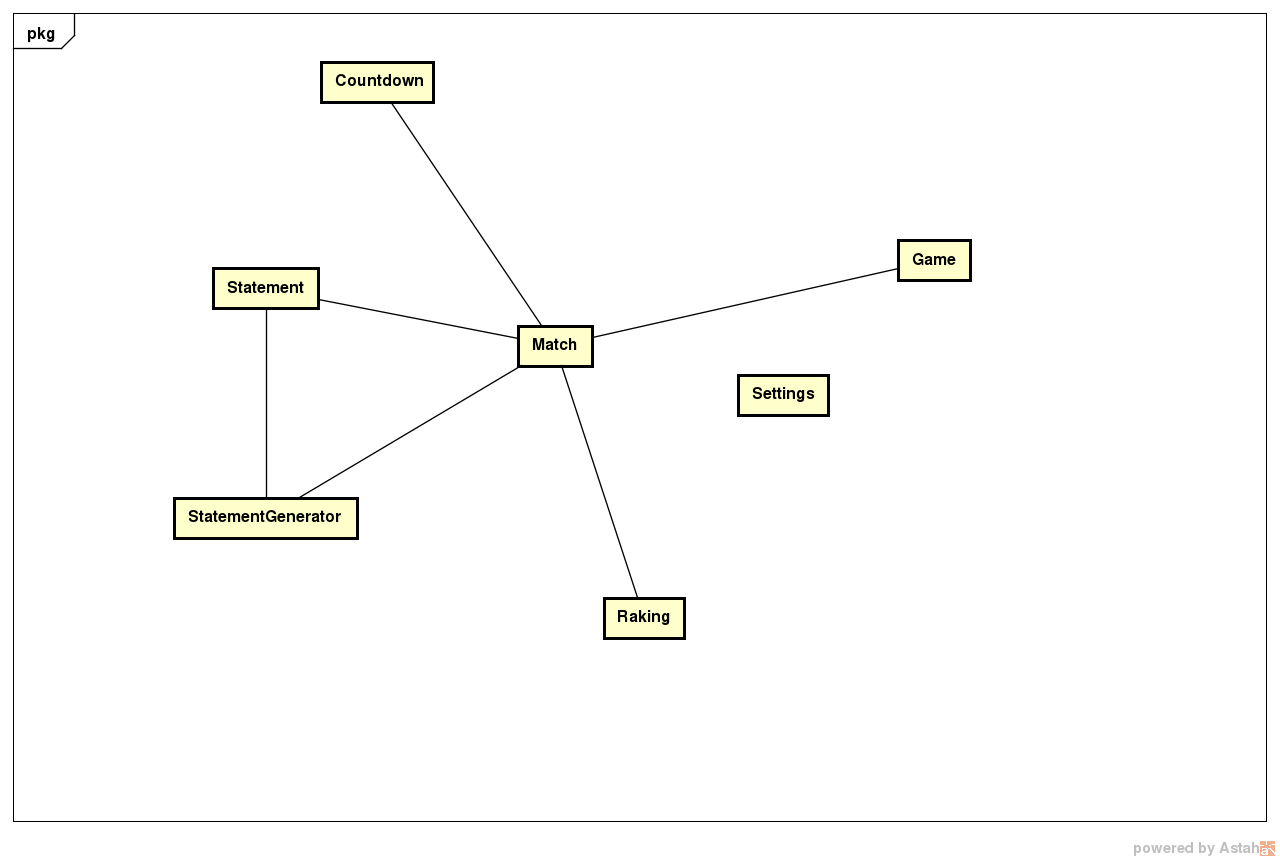
\includegraphics[width=0.8\textwidth,natwidth=610,natheight=642]{ClassesSimpleView.png}
	\caption{Diagrama de classes simplificado}
\end{figure}

\begin{draft}
\section{Desenvolvimento}

O desenvolvimento se deu com uma postura de melhoria progressiva.
Desenvolvendo a versão mais simples possível para atingir as
requisitos funcionais. A partir dessa versão, novos recursos foram
sendo adicionadas para melhorar a experiência do usuário.

O primeiro passo foi a criação do documento HTML. Utilizei divs
para simbolizar telas do jogo. Caracterizando o jogo como uma
aplicação de uma única página (\textit{Single Page Application}).
Alternativamente poderia se depender de um servidor para mandar as
páginas prontas, mas isso distribui a complexidade do sistema para
tecnologias do lado do servidor, distanciando-se da proposta de jogos
exclusivamente construídos com as tecnologias da WEB.

Seguindo a construção do documento HTML, veio o desenvolvimento de um
CSS simples que comporta a visualização em múltiplos dispositivos.
Para tal, foram utilizadas posições e tamanhos relativos. Por exemplo,
a largura de cada tela da SPA é 98\% do tamanho total disponível na
tela. Já o tamanho da fonte do quadro principal, representado pelo id
\textit{billboard} é duas vezes o tamanho da fonte normal 2em.

Sem a ajuda de bibliotecas especializadas o processo de criação da
interface não é trivial. Apesar de a interface ser simples, fazer os
elementos se alinharem em diversos tamanhos de telas não é fácill e
pode se tornar um grande problma para interfaces realmente complexas.

Após a concepção do CSS deu-se início ao desenvolvimento da lógica do 
negócio em JavaScript. O primeiro passo consistiu em fazer o mecanismo 
de múltiplas telas em JavaScript. Ao iniciar a execução do JavaScript
todas as divs que representam telas foram escondidas. O script mostra
em seguida a página de carregamento. No final do carregamento de todos 
os recursos é disparado o evento \textit{window.onload} neste momento
inicia-se uma partida. Foram adicionados  \textit{listeners} os eventos de 
clicar nas configurações e nos botões de certo e errado da página principal, 
o botão de configurações simplesmente esconde todas as seções  e por fim carrega
a de configurações. Os botões de certo e errado serão explicados na sequência.

Após o esqueleto da aplicação estar definido foi introduzido a lógica de negócio.
De toda a regra do jogo, a classe Match é a mais importante.
Ela simboliza uma partida dentro do jogo, é na classe Match que 
as informações de quantas equações existem, quantas foram acertadas
e o tempo total da partida e sua pontuação. Seu propósito é iterar 
a cada pergunta e esperar por uma resposta. Quando a resposta é dada
a classe Match computa se a resposta está correta ou não e o tempo 
que levou para chegar ao resultado. Quando não existem mais perguntas 
para serem processadas é lançado um evento de final de partida onde 
o resultado pode ser computado, demostrado para o usuário e registrado 
no ranking.

No nesta etapa não havia um gerador de equações, o jogo
contava apenas com uma coleção de equações preestabelecidas que eram
selecionadas aleatoriamente a cada turno. Isso se provou uma boa escolha
pois possibilitou que o desenvolvimento se focasse em outros aspectos
importantes como a elaboração do laço do jogo, ranking, configurações entre outros.

O ranking serve para armazenar o resultado de cada partida do jogador
possibilitando uma percepção de histórico da performance do jogador.
Os dados são armazenados em Local Storage, escolhido por
ter uma API simples; visto que os requerimentos do protótipo não
demandam grande performance ou armazenamento massivo de dados a opção
mais modesta foi preferida. Arquiteturalmente falando, IndexedDb se
encaixaria bem na aplicação por ter uma interface chave valor,
ideal para um ranking, onde as chaves poderiam ser as posições do usuário,
não obstante, a interface totalmente orientada a eventos do IndexedDb
introduz uma complexidade desnecessária para um jogo simples.
A classe ranking é simplesmente uma interface para converter partidas e armazenar
e recuperas estas informações em Local Storage.

O objeto \textit{Settings}, assim como o Ranking, utiliza Local Storage
e provê uma interface para armazenar e recuperar preferências sobre o jogo.
Cada campo editável na tela de configurações contém listeners prontos
para registrar no objeto \textit{Settings} cada mudança que ocorrer em seus estados.
Os objetos que utilizam estas configurações também o fazem através do objeto settings
então a validade das configurações é sempre garantida.

Implementados estes mecanismos essenciais para o jogo, pude me focar no
ponto centra do negócio e possivelmente o mais possivelmente o mais
complexo: a geração de equações. As geração das equações envolve
dois objetos. Um objeto \textit{Statement}, responsável por armazenar
as informações de uma equação, à dizer: a afirmação sendo feita e
se seu resultado está correto ou não (a reposta da afirmação).
O outro objeto envolvido neste processo é o \textit{StatementGenerator},
responsável por gerar \textit{Statements}.

A classe \textit{StatementGenerator} conta com um método
\textit{getStatement} que realiza o processamento para gerar um novo
\textit{Statement}. Esta função recebe como argumento um inteiro que
simboliza a dificuldade da equação, a cada iteração do usuário
armazenada no objeto \textit{Match} a dificuldade é incrementada
e repassada para o gerador. O valor da dificuldade é utilizado
internamente no para selecionar qual operador será utilizado e como
multiplicador nos números componentes das equações. Superficialmente
falando, as equações são geradas através da randomização de
valores e operadores (com suas respectivas dificuldades processadas),
seguido da execução da equação para determinar seu resultado e a
geração, em 50\% dos casos, de um valor errado, de modo que a resposta
não seja sempre correta. 

O objeto \textit{StatementGenerator} reside como membro de classe
do objeto \textit{Match} e a cada interação com o usuário
uma nova equação é gerada por ele e armazenada no atributo
\textit{currentStatement} do objeto \textit{Match}. Ao final das iterações com
o usuário o evento \textit{endOfMatch} é lançado onde os pontos são
computados, armazenados e mostrados para o usuário. Neste ponto é
possível também começar outra partida reiniciando o processo.

Estas classes comportam os requisitos funcionais do jogo. Ao final
do processo foi identificado que muitas vezes o usuário começa uma
partida e não está prestando atenção para a tela perdendo pontos
neste período inicial. Para reduzir este problema foi adicionada 
a classe \textit{Countdown}, que é basicamente um temporizador regressivo que 
demarca o início de cada partida. O temporizador foi desenvolvido em canvas
e apresenta 4 demarcações desenhadas a cada 90 graus, formando um circulo com uma
mensagem no centro, neste caso os números do temporizador.

%posteriori
Uma estratégia interessante que foi adotada na construção foi
declarar todos os objetos relativos ao objeto janela (\textit{window}).
Isso se demonstrou uma boa forma de separar os objetos, tornando o
conflito de variáveis globais um problema irrelevante.

Outro aspecto positivo foi a utilização de um meta objeto para
encapsular os demais, neste caso utilizei o nome MyMath, funcionando
como um namespace, garantindo que problemas de conflitos de nomes não
aconteçam.

\end{draft}
\begin{figure}
    \centering
    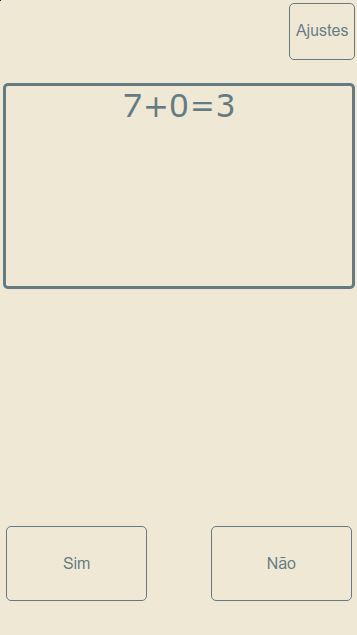
\includegraphics[width=0.8\textwidth,natwidth=610,natheight=642]{board.png}
	\caption{Tabuleiro do jogo com equação sendo apresentada}
    \label{fig:tabuleiro}
\end{figure}

\begin{figure}
    \centering
    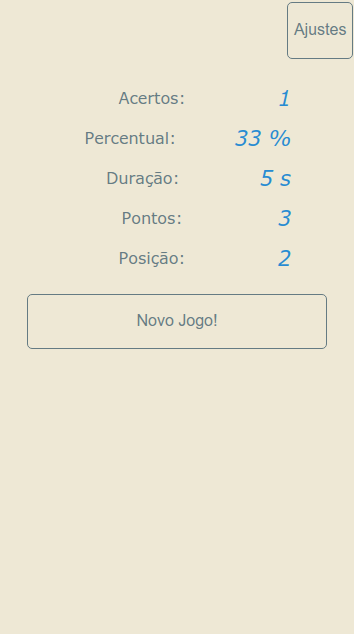
\includegraphics[width=0.8\textwidth,natwidth=610,natheight=642]{score.png}
	\caption{Placar do jogo}
\end{figure}

\begin{figure}
    \centering
    
\includegraphics[width=0.8\textwidth,natwidth=610,natheight=642]{settings.png}
	\caption{Configurações do jogo}
\end{figure}

\begin{draft}

\section{Otimizações para jogos}

Navegadores tentam otimizar a experiência de navegação definindo
um conjunto de regras e configurações razoáveis para a maioria dos
casos. Não obstante, nem sempre estes valores padrões são as melhores
opções no contexto de jogos. Abaixo segue uma lista de configurações
interessantes para se fazer com CSS no contexto de desenvolvimento de
jogos.
Abaixo seguem algumas otimizações que foram utilizadas no jogo, e são  aplicáveis 
em grande parte dos jogos.

\subsection{CSS}

Scroll é um recurso interessante para longas páginas de texto,
o mesmo não se pode dizer à respeito de jogos.
Principalmente aqueles dependente de contato com a tela, pois
no contato a tela pode se mover e desconcentrar o usuário. Para
remover este comportamento deve-se utilizar o \textit{overflow:
hidden;} do seletor do corpo do documento (\textit{body}).

A barra de endereço é outro recurso de pouca utilidade no contexto de
jogos, e muitas vezes um empecilho para jogos em dispositivos móveis,
devido ao limitado tamanho da tela.

Para desabilitar a barra em dispositivos da Apple pode-se utilizar a
seguinte configuração:

\begin{verbatim}
<meta name="apple-mobile-web-app-capable" content="yes" />
\end{verbatim}

Para os demais dispositivos não existe meio oficial de esconder a barra
de endereço. Não obstante, alguns sites recomendam a solução descrita abaixo:

\begin{verbatim}
<body onload="setTimeout(function() {window.scrollTo(0, 1)}, 100)">
</body>
\end{verbatim}

Apesar de não fazer parte da especificação, a maioria dos navegadores
implementa a possibilidade de desativar a seleção de elementos na tela.
Em jogos essa possibilidade é útil, pois não é natural a seleção de texto
neste tipo de software. \cite{html5mostwanted} cita que desabilitar
a seleção de texto em jogos é uma otimização importante para a
experiência do usuário. Para desabilitar pode-se utilizar as regras
CSS demonstradas abaixo.

\begin{verbatim}
-moz-user-select: none;
-webkit-user-select: none;
-ms-user-select: none;
\end{verbatim}

\subsection{JavaScript}
\subsubsection{Modo estrito}
Algumas das recomendações nesta seção podem não se aplicar
exclusivamente ao desenvolvimento de jogos. Outrossim são de grande
relevância para a criação de sistemas de grande complexidade em geral,
característica comum da grande maioria dos jogos.

Um recurso interessante do JavaScript é seu modo estrito, este faz
um conjunto de modificação na semântica do interpretador de modo
que alguns recursos suportados, mas propensos a problemas, sejam
desabilitados. Um exemplo é variáveis sem o prefixo var.

O modo estrito pode ser entendido como uma variante mais rígida
do JavaScript. O modo restrito pode ser habilitado utilizando o
termo \textit{"use strict";} nos cabeçahos de arquivos ou funções
permitindo que código não estrito trabalhe em conjunto com código
estrito, característica conveniente para a utilização em sistemas
legados.

\subsubsection{Funções imediatamente invocadas}

Um problema comum de sistemas complexos em JavaScript é que muitos
objetos vivem em ambiente global. Isso pode causar uma coleção de
problemas, desde conflitos de nomes à sobrescrita de variáveis. Para
contornar esse problema pode-se utilizar as funções imediatamente
invocadas IFE (\textit{Immediatly invoked function expression}).
\end{draft}

\begin{figure}
\centering
\begin{verbatim}
    (function() {
        'use strict';

        function bar() {
            return 'foo';
        }

        window.bar = bar;
    })();
    window.bar();
\end{verbatim}
\caption{Exemplo de utilização de funções imediatamente invocadas}
\label{fig:iife}
\end{figure}
\begin{draft}

A figura \ref{fig:iife} demonstra a utilização deste padrão. As
funções definidas no mesmo nível que bar não estarão no contexto
global - a não ser que seja especificado diretamente - e não sofrerão
conflitos de nomes e outros problemas relativos ao contexto global.

\subsubsection{HTML}

Um problema que jogos sofrem em geral é a demora no carregamento da
grande quantidade de recursos que precisam estar em memória para o jogo
funcionar. Muitos jogos utilizam uma tela de carregamento enquanto os 
recursos são adquiridos.

Um recurso do HTML interessante para este tipo de situação é o pré
carregamento de recursos (\textit{Link Prefetching}). Esta tecnologia
possibilita que o navegador , em seu tempo livre, adquira recursos que
provavelmente serão necessários em um futuro próximo.

Nem todos os recursos necessitam ser pré carregados, mas uma impressão
muito superiora é criada se os recursos estão imediatamente
disponíveis quando uma nova fase é carregada \autocite[pp. 39]{creatingFun}.

\section{Performance}

O jogo ficou rápido...

\end{draft}
